\chapter{\system}
\label{chap:lazarus_implementation}
This chapter presents \system iplementation, these mechanisms were implemented to be fully automated, removing the human from the loop.
The current implementation of \system manages 17 \gls{os} versions, supporting the \gls{bft} replication of a set of representative applications.
The replicas run in \glspl{vm}, allowing provisioning mechanisms to configure them. 
We conducted two sets of experiments, one demonstrates that \system risk management can prevent a group of replicas from sharing vulnerabilities over time; the other, reveals the potential negative impact that virtualization and diversity can have on performance. However, we also show that if naive configurations are avoided, \gls{bft} applications in diverse configurations can actually perform close to our homogeneous bare metal setup.
%These results open avenues for many future works in the area. 


\section{Implementation}
\label{sec:implementation}

This section details the implementation of each component of \system. 
It also briefly presents other aspects of our prototype.% like the management of replicas running in a virtualized environment.


\subsection{Control Plane}
\label{sec:lazarus}

Figure~\ref{fig:arch1} shows \system control plane with its four main modules, described below.

\begin{figure}[h]
\begin{center}
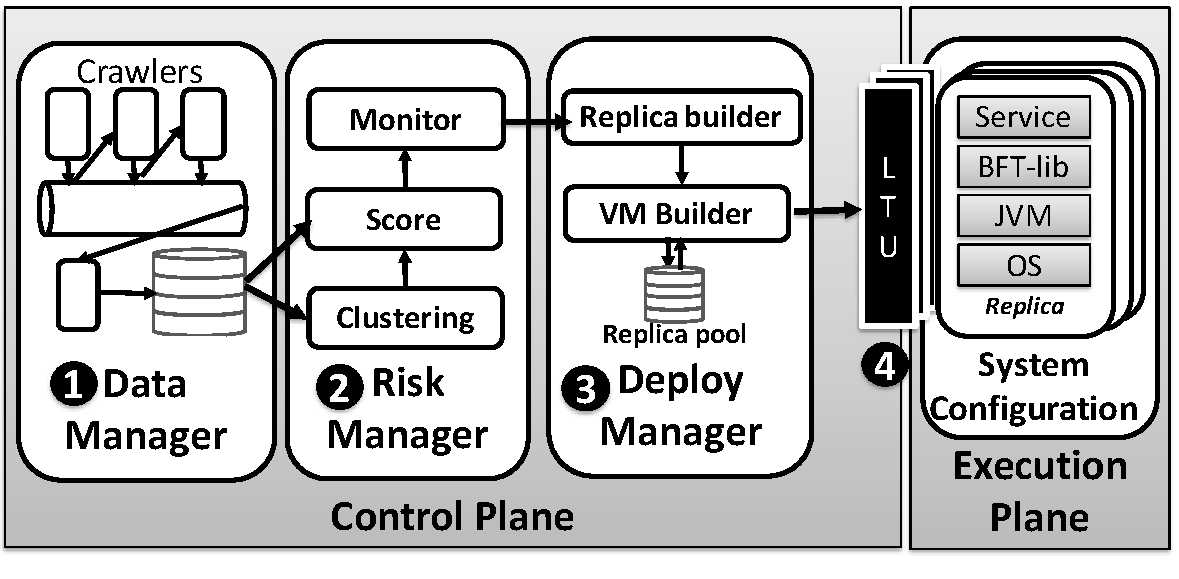
\includegraphics[width=.9\columnwidth]{images/images/architecture_new.pdf}
\vspace{-5mm}
\caption{\system architecture.}
\vspace{-5mm}
\label{fig:arch1}
\end{center}
\end{figure}


\circled{1} \textbf{\fetcher.} \system needs to know the software stack of each available replica to be able to look for vulnerabilities in this software.
The list of software products is provided following the \gls{cpe} Dictionary~\cite{cpe}, which is also used by \gls{nvd}. 
%The \fetcher determines if the CPE list is updated by checking the most recent CPE count in the NVD web page.
For each software, the administrator can indicate the time interval (in years) during which data should be obtained from \gls{nvd}' feeds.

The \fetcher parses the \gls{nvd} feeds considering only the vulnerabilities that affect the chosen products. 
The processing is carried out with several threads cooperatively assemblying as much data as possible about each vulnerability -- a queue is populated with requests pertaining a particular vulnerability, and other threads will look for related data in additional \gls{osint} sources. 
Typically, the other sources are not as well structured as \gls{nvd}, and therefore they have to be handled with specialized HTML parsers that we have developed. 
Currently, the prototype supports five other sources, namely Exploit DB, CVE-details, Ubuntu, Debian, and Microsoft. 
As previously mentioned, such sources provide complementary data, like additional affected products versions not mentioned in \gls{nvd}.

The collected data is stored in a relational database (MySQL).
For each vulnerability we keep its \gls{cve} identifier, the published date, the products it affects, its text description, some \gls{cvss} attributes (e.g., availability and integrity); and exploit and patching dates.


\circled{2} \textbf{\risk.} This component finds out when it is necessary to replace the currently running group of \replicas and discovers an alternative configuration that decreases the risk. 
As explained in Section~\ref{sec:measurerisk}, the risk is computed using score values that require two kinds of data: the information about the vulnerabilities, which is collected by the \fetcher; and the vulnerability clusters. 
A vulnerability cluster is a set of vulnerabilities that are related accordingly to their description (see Section~\ref{sec:details} for details).
The \risk also runs Algorithm~\ref{alg:algorithm2} to monitor the replicated system and trigger reconfigurations.


\circled{3} \textbf{\manager.} 
This component automates the setup and execution of the diverse replicas. 
It creates and deploys the \replicas in the execution environment implementing the decisions of the \risk, i.e., it dictates when and which \replicas leave and join the system. 
We developed a replica builder on top of Vagrant~\cite{vagrant}.
It is responsible for downloading, installing, and configuring the \replicas.
Moreover, it performs replica maintenance, where  \replicas in \QS are booted to carry out automatic software updates (i.e., patching). 


\paragraph{Setup.}
The box configuration is defined in a configuration file, named \emph{Vagrantfile}, consider the example in Listing~\ref{vagrantfile}.
In this file, it is possible to set several options of the box, to name a few:
the box name, the number of CPUs, the amount of memory RAM, the IP, the type of network, sync folders between host and the box, etc. 
Additionally, it is possible to pass some VM-specific parameters, e.g., some CPU/mother board flags such as enabling VT-x technology -- consider the \texttt{modifyvm} fields in Listing~\ref{vagrantfile} (lines 6-14).
It is possible to select different \gls{vm} providers (e.g., libvirt, VMware, VirtualBox, Parallels, Docker, etc), we rely on VirtualBox since it is the one with more diversity opportunities in the Vagrant Cloud~\cite{vagrantcloud}. 
Vagrant Cloud is a website that offers a plethora of different VMs.

\begin{lstlisting}[style=mystyle,caption=Windows Server 2016 Vagrantfile,label=vagrantfile]
Vagrant.configure(2) do |config|
	config.vm.box = "geerlingguy/ubuntu1604"
	config.ssh.insert_key = false
	config.vm.provider "virtualbox" do |v|
		v.customize ["modifyvm", :id, "--cpus", 4]
		v.customize ["modifyvm", :id, "--memory", 22000]
		v.customize ["modifyvm", :id, "--cpuexecutioncap", 100]
		v.customize ["modifyvm", :id, "--ioapic", "on"]
		v.customize ["modifyvm", :id, "--hwvirtex", "on"]
		v.customize ["modifyvm", :id, "--nestedpaging", "on"]
		v.customize ["modifyvm", :id, "--pae", "on"]
		v.customize ["modifyvm", :id, "--natdnshostresolver1", "on"]
		v.customize ["modifyvm", :id, "--natdnsproxy1", "on"]
	end
	config.vm.network "public_network", ip:"192.168.2.50", bridge:"em1"
	config.vm.provision :shell, path: "run_debian.sh", privileged: true
end
\end{lstlisting}

\todo{Add all fields that are mentioned, then add lines to the text}

\paragraph{Download.}
One of the fields of the \emph{Vagranfile} is the boxname, the \texttt{box} field is the key that is used to choose which box will be downloaded, each key is unique for each box.
There are plenty of \glspl{os} and versions ready-to-use, and the same OS/version can have different ``manufacturers" -- some of which are official.

\paragraph{Deploy and provision.}
Vagrant supports complex provisions mechanisms, such as Chef or Puppet, but shell script was sufficient for us. 
This is set in the \emph{Vagranfile} \texttt{provision} field, one can describe the provision steps inline or in an external file and link it to the \emph{Vagranfile}.
Then, when the OS is booting, after the basic setup, the \glspl{os} will execute the provision script.
In this script, we program which software will be downloaded and run in the \glspl{vm} and what configurations are needed. 
We have developed shell scripts for each \glspl{os}, some of which share the same script as Debian and Ubuntu. 
Each \glspl{os}, especially the ones from different \glspl{os} families (e.g., Solaris and BSD) have different commands to execute the same instructions.
Although different, all scripts were meant to do the same thing:
First the script installs the software that is missing in the box -- this is not true for all OSes -- like Java 8, \texttt{wget}, \texttt{unzip}, and any additional software that one wants to install/run after the \glspl{os} boot.



\paragraph{Command and Control.}
There are some simple commands to boot and halt a box, e.g., \texttt{vagrant up} and \texttt{vagrant halt}. 
Vagrant also provides an ssh command (\texttt{vagrant ssh}) that allows the host to connect to the box. 
Our manager component makes the bridge between the \risk and the execution environment.
We developed an API on top of Vagrant, another level of abstraction made to manage replicated systems.


\circled{4} \textbf{LTUs.} Each node that hosts a replica has a Vagrant daemon (see details in next section) running on its trusted domain.
This component is isolated from the internet and communicates only with the \system controller through \gls{tls} channels.

\subsection{Additional Details}
\label{sec:details}

\textbf{Vulnerability Clustering.}
A few steps are carried out to create the vulnerability clusters. 
First, the vulnerability description needs to be transformed into a vector, where a numerical value is associated with the most relevant words (up to 200 words). 
This operation entails, for example, converting all words to a canonical form and calculating their frequency (less frequent words are given higher weights).
Then, the K-means algorithm is applied to build the clusters~\cite{Jain:2010}, where the number of clusters to be formed is determined by the elbow method~\cite{Thorndike:1953}. 
%Currently, it is set $K=200$.
%The algorithm assigns each vulnerability to the cluster with the minimum distance to the cluster center. 
%Then, it computes the cluster centroid, i.e., the average of each data attribute using only the members of a cluster. 
%Next, it calculates the distance of every vulnerability to the centroid, potentially placing them in close clusters. 
%The algorithm stops when there are no further exchanges between clusters.
%We used the elbow method~\cite{Thorndike53whobelongs} to determine the number of clusters to be formed, in our case was $200$ clusters.
We used the open-source machine learning library Weka~\cite{weka} to build the clusters. 


\subsection{Clustering}\label{sec:clustering}
Clustering is the process of aggregating elements into similar groups, named clusters. 
For example, two elements from the same cluster have a higher probability of being similar than two elements from different clusters. 
We apply this technique to build clusters of similar vulnerabilities.
One of the benefits of applying clustering techniques to vulnerability-data is that the algorithm does not need prior knowledge about the data.
It is the process alone that discovers the hidden knowledge in the data.
Each cluster is used as a hint that similar vulnerabilities are likely to be activated through the same or similar exploit.
We considered the vulnerability description and published date to find these similarities. 
In the end, it is expected that the clusters have a minimal number of elements that just represent the same or similar vulnerabilities.


In order to apply a clustering technique to our data, we need to follow some steps:

\paragraph{1) Data representation}
We transform the data that is stored in a database into a format that is readable by the clustering algorithm. 
Since we are using Weka~\cite{weka}, the data must be represented as \gls{arff}. 
Basically, this is a CSV file with some meta information, see Listing~\ref{list:arff}.

\begin{lstlisting}[style=mystyle,caption=ARFF file describing a vulnerability.,label=list:arff]
@RELATION vulnerabilities
@ATTRIBUTE cve string
@ATTRIBUTE description string
@ATTRIBUTE published_date date "yyyy-MM-dd"
@DATA
CVE-2017-3301, 'vulnerability in the solaris component of oracle sun systems products suite subcomponent kernel the supported version that is [...] attacks of this vulnerability can result in unauthorized update insert or delete access to some of solaris accessible data cvss v base score integrity impacts', '2017-01-27'
...more
\end{lstlisting}


This file contains all the vulnerabilities entries in the database. 
As we are interested in the vulnerability similarities, we select only the \gls{cve} identifier, the text, that contains the most relevant and nonstructured information, and the published date.
These attributes add meaning and temporal reference to the clustering algorithm.


\paragraph{2) Data preparation}
In general, machine learning algorithms do not handle raw data, then the data needs to be prepared:
First, we transform the \gls{cve} string into a number, basically, for each \gls{cve}, there is a real number that identifies each \gls{cve} unequivocally. 
This attribute is transformed in numeric values using \emph{StringToNominal} filter. 
Each \gls{cve} identifier is mapped to a numeric value.
Second, we transform the published date to a number format that Weka can handle using the \emph{NumericToNominal} filter.
Third, the text description must be transformed into a vector, the vector will represent the frequencies of each word in the whole document of strings. 
We used the \emph{StringToWordVector} to transform a text string into a vector of word weights, these weights represent the relevance of each word in the document.
This filter contains the following parameters:
\begin{itemize}
\item \textbf{TF- and IDF-Transform}, both set to true, TF-IDF stands for term frequency-inverse document frequency. 
This is a statistical measure used to evaluate how relevant a word is to a document in a collection. 
The relevance increases proportionally to the number of times a word appears in the document but is offset by the frequency of the word in the corpus. 
For example, words that appear in all vulnerability descriptions, are less relevant than the ones that appear more in few vulnerabilities.
\item \textbf{lowerCaseTokens}, convert all the words to lower case.
\item \textbf{minTermFreq}, set to -1, this will preserve any word despite their occurrences in the document.
\item \textbf{normalizeDocLength}, set to normalize all data.
\item \textbf{stopwords}, we define a stop word list, then words from this list are discarded. We begin with a general English stop word list containing pronouns, articles, etc. 
\item \textbf{tokenizer}, set to \emph{WordTokenizer}, this filter will remove special characters from the text, there is a default set of characters but we added a few more.
\item \textbf{wordsTopKeep}, is the number of words that will be kept to make the clusters. We kept $200$ as it was the number of words that represent better the lexical of vulnerabilities after removing the \emph{stopwords}.
\end{itemize}


Our goal is to build clusters in such way that similar vulnerabilities, even if they affect different products, are put together in the same cluster. 
For example, recall the vulnerabilities in Table~\ref{tab:missing_products}, which can be put in the same cluster since they are very similar.
Some of the parameters listed above needed some tuning to achieve our goals.
For example, before the tuning, some of the clusters were representing types of vulnerabilities, e.g., buffer overflow, cross-site scripting, etc. 
Since we are not interested in that type of clusters we have refined our \emph{stopword list} to reduce the description vocabulary to contain only what matters for us.
We have done this by iterating the process and checking the most used words (top 200 words) for clustering (this can be seen in Weka's intermediary output).
Then, we added the most relevant from the 200 words that were deviating from our goal.
In the end, we have a stop word list~\footnote{Stop word list is available: here} without the security-vocabulary noise.


When the pre-filtering ends, Weka presents a file very similar to the previous \gls{arff} file with the difference that the features are the most relevant words in the corpus. And each instance contains a value of relevance for each word.


\paragraph{3) Making clusters}
K-means is an unsupervised machine learning algorithm that groups data in K clusters.
The \emph{K-means} has two important parameters: the number of clusters to be formed, we set to $200$ clusters. We used the elbow method~\cite{Thorndike:1953} to decide $k=200$; and the \emph{distance function}, to calculate the distance between objects, the \emph{Euclidean Distance} is the most adequate for this type of data;
The \emph{K-means} computes the distance from each data entry to the cluster center (randomly selected in the first round).
Then, it assigns each data entry to a cluster based on the minimum distance (i.e., Euclidean distance) to each cluster center.
Then, it computes the centroid, that is the average of each data attribute using only the members of each cluster.
Calculate the distance from each data entry to the recent centroids. 
If there is no modification (i.e., re-arrangement of the elements in the cluster), then the clusters are complete, or it recalculates the distance that best fits the elements. 
When the K-means finishes the execution, we take the cluster assignments of each vulnerability. 
The assignments will be added to a new \gls{arff} file, similar to the first one but with a new attribute that is the cluster name (e.g., cluster1, cluster2, etc). 



Sometimes the resulting clusters include vulnerabilities that are unrelated. Therefore, we use the Jaccard index (J-index) to measure the similarity between the vulnerabilities within the cluster. We calculate the J-index of each element, and then the average J-index of the cluster. 
The clusters with a smaller average J-index (below a certain threshold) are considered ill-formed. In this case, we select the vulnerabilities with lower J-index and move them to another cluster that would result in a better J-index. If no such cluster exists, then we create a new one with the ``orphan'' vulnerability.

\textbf{BFT replication.}
Although there has been relevant research on \gls{bft} protocols over the last twenty years, there are few open-source replication libraries that implement them. \system can use any of those libraries, as long as they support replica set reconfigurations.
More specifically, to manage the \replicas, we need the ability to add first a new \replica to the set and then remove the old \replica to be quarantined. 
Therefore, we employ BFT-SMaRt~\cite{Bessani:2014}, a stable \gls{bft} library that provides reconfigurations on the \replicas set.

\textbf{Replica Virtualization.}
\glspl{vm} can be used to implement replicated systems, leveraging on the isolation between the untrusted and the trusted domains~\cite{Sousa:2010,Platania:2014,Distler:2011,Dettoni:2013}.
Recovery triggering can be initiated from the isolated domain in a synchronous manner, reducing the downtime of the service during the reconfigurations. 
In our implementation, we resort to the Vagrant~\cite{vagrant} provisioning tool to do fast deployment of ready-to-use \glspl{os} and applications on \glspl{vm}. 
Vagrant supports several virtualization providers, e.g., VMware and Docker. 
From the available alternatives, we chose VirtualBox~\cite{virtualbox} because it offers more diversity opportunities, i.e., it supports a more extensive set of different guests \glspl{os}.
%The VMs are available in the Vagrant Cloud~\cite{vagrantcloud}.

\subsection{Descentralized \system Version}

\section{Performance Evaluation}
\label{sec:overhead}

In this section, we evaluate how \system' affects the performance of diverse replicated systems.
First, we run the BFT-SMaRt microbenchmarks in our virtualized environment using 17 \gls{os} versions to understand how the performance of a \gls{bft} protocol varies with different \glspl{os}, and how they compare with the performance of a homogeneous bare metal setup.
Second, we use the same benchmarks to measure the performance of specific diverse setups.
Third, we analyze the performance of the system along \system-managed reconfigurations.
Fourth, we measure the time that each OS takes to boot.
Finally, we evaluate the performance of three \gls{bft} services running in the \system infrastructure.


These experiments were conducted in a cluster of Dell PowerEdge R410 machines, where each one has 32 GB of memory and two quad-core 2.27 GHz Intel Xeon E5520 processor with hyper-threading, i.e., supporting 16 hardware threads on each node.
The machines communicate through a gigabit Ethernet network.
Each server runs Ubuntu Linux 14.04 LTS (3.13.0-32-generic Kernel) and VirtualBox 5.1.28, for supporting the execution of VMs with different OSes. 
Additionally, Vagrant 2.0.0 was used as the provisioning tool to automate the deployment process.
In all experiments, we configure BFT-SMaRt v1.1 with four replicas ($f=1$), one replica per physical machine.

Table~\ref{tab:oses} lists the 17 \gls{os} versions used in the experiments and the number of cores used by their corresponding \glspl{vm}.
These values correspond to the maximum number of CPUs supported by VirtualBox with that particular \gls{os}.
The table also shows the \gls{jvm} used in each \gls{os}, and the amount of memory supported by each of these \glspl{vm}.
Given these limitations we setup our environment to establish a fair baseline by configuring an \emph{homogeneous} \gls{bm} environment that uses only four cores of the physical machine. 

%Given the limitations of the VMs we were able to setup in our environment, all experiments conducted in our \emph{homogeneous bare metal environment} (BM) were configured to make BFT-SMaRt replicas use only four cores of the machines, to establish a fair baseline.


\begin{table}[t]
\begin{center}
{\footnotesize
\begin{tabular}{| c | c | c | c | c |}\hline
\textbf{ID} & \textbf{Name}  & \textbf{Cores} & \textbf{JVM} & \textbf{Mem.} \\\hline\hline
UB14 & Ubuntu 14.04 & 4 & Java Oracle 1.8.0\_144 & 15GB \\ \hline
UB16 & Ubuntu 16.04 & 4 & Java Oracle 1.8.0\_144 & 15GB \\ \hline
UB17 & Ubuntu 17.04 & 4 & Java Oracle 1.8.0\_144 & 15GB \\ \hline
OS42 & OpenSuse 42.1 & 4 & Openjdk 1.8.0\_141 & 15GB \\ \hline
FE24 & Fedora 24 & 4 & Openjdk 1.8.0\_141 & 15GB \\ \hline
FE25 & Fedora 25 & 4 & Openjdk 1.8.0\_141 & 15GB \\ \hline
FE26 & Fedora 26 & 4 & Openjdk 1.8.0\_141 & 15GB \\ \hline
DE7 & Debian 7 & 4 & Java Oracle 1.8.0\_151 & 15GB \\ \hline
DE8 & Debian 8 & 4 & Openjdk 1.8.0\_131 & 15GB \\ \hline
W10 & Windows 10 & 4 & Java Oracle 1.8.0\_151 &1GB \\ \hline
WS12 & Win. Server 2012 & 4 & Java Oracle 1.8.0\_151 & 1GB \\ \hline
FB10 & FreeBSD 10 & 4 & Openjdk 1.8.0\_144 & 15GB \\ \hline
FB11 & FreeBSD 11 & 4 & Openjdk 1.8.0\_144 & 15GB \\ \hline
SO10 & Solaris 10 & 1 & Java Oracle 1.8.0\_141 & 15GB \\ \hline
SO11 & Solaris 11 & 1 & Java Oracle 1.8.0\_05 & 15GB \\ \hline
OB60 & OpenBSD 6.0 & 1 & Openjdk 1.8.0\_72 & 1GB \\ \hline
OB61 & OpenBSD 6.1 & 1 & Openjdk 1.8.0\_121 & 1GB \\ \hline
\end{tabular}
}
\caption{The different OSes used in the experiments and the configurations of their VMs and JVMs.}
\label{tab:oses}
\end{center}
\end{table}


\subsection{Homogeneous Replicas Throughput}


We start by running the BFT-SMaRt microbenchmark using the \emph{same \gls{os} version} in all replicas.
The microbenchmark considers an empty service that receives and replies variable size payloads, and is commonly used to evaluate \gls{bft} state-machine replication protocols (e.g., \cite{Castro:1999,Bessani:2014,Liu:2016,Behl:2015,Behl:2017}). 
Here, we consider the $0/0$ and $1024/1024$ workloads, i.e., $0$ and $1024$ bytes requests/response, respectively.
The experiments employ up to 1400 client processes spread on seven machines to create the workload.
% and the throughput was measured in the BFT-SMaRt leader replica.

\textbf{Results:}
Figure~\ref{fig:bftsmart} shows the throughput of each \gls{os} running the benchmark for both loads.
To establish a baseline, we executed the benchmark in our bare metal Ubuntu, without \system virtualization environment.

The results show that there are some significant differences between running the system on top of different \glspl{os}.
This difference is more significant for the $0/0$ workload as it is much more CPU intensive than the $1024/1024$ workload.
Ubuntu, OpenSuse, and Fedora OSes are well supported by our virtualization environment and achieved a throughput around $40k$ and $10k$ for the $0/0$ and $1024/1024$ workloads, which corresponds to approx. $66\%$ and $75\%$ of the bare metal results, respectively.
For Debian, Windows, and FreeBSD, the results are much worse for the CPU intensive $0/0$ workloads but close to the previous group for $1024/1024$.
Finally, single core VMs running Solaris and OpenBSD reached no more than $3000$ ops/sec with both workloads.

These results show that the virtualization platform limitations on supporting different \glspl{os}, strongly limits the performance of specific \glspl{os} in our testbed.

\begin{figure}[h]
\begin{center}
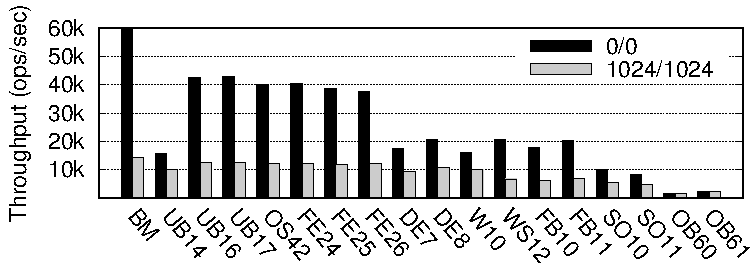
\includegraphics[width=\columnwidth]{images/gnuplot/vagrant/runs_new_new/throughput.pdf}
\caption{Microbenchmark for 0/0 and 1024/1024 (request/replying) for homogeneous OSes configurations.}
\label{fig:bftsmart}
\end{center}
\end{figure}

\subsection{Diverse Replicas Throughput}
\label{sec:performancediversity}

The previous results show the performance of BFT-SMaRt when running on top of different \glspl{os}, but with all replicas running in the same environment.
In this experiment, we evaluate three diverse sets of four replicas, one with the fastest \glspl{os} (UB17, UB16, FE24, and OS42), another with one replica of each \gls{os} family (UB16, W10, SO10, and OB61), and a last one with the slowest \glspl{os} (OB60, OB61, SO10, and SO11).
The idea is to set an upper and lower bound on all possible diverse sets throughput.

\begin{figure}[h]
\begin{center}
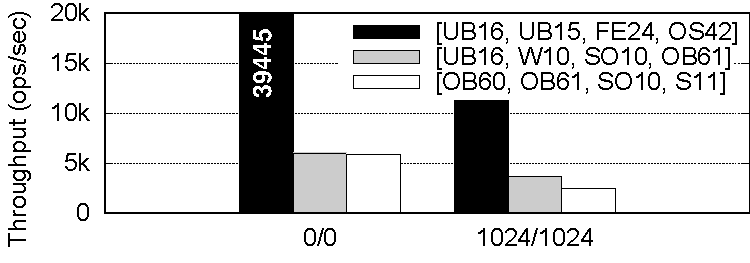
\includegraphics[width=\columnwidth]{images/gnuplot/vagrant/runs_diversity/throughput.pdf}
\caption{Microbenchmark for 0/0 and 1024/1024 (request/reply) for three diverse OS configurations.}
\label{fig:diversets}
\end{center}
\end{figure}


\textbf{Results:}
Figure~\ref{fig:diversets} shows that throughput drops from 39k to 6k for the $0/0$ workload ($65\%$ and $10\%$ of the bare metal performance), and from 11.5k to 2.5k for the $1024/1024$ workload ($82\%$ and $18\%$ of the bare metal performance).
When comparing these two sets with the non-diverse sets of Figure~\ref{fig:bftsmart}, the fastest set is in $7^{th}$, and the slowest set is in $16^{th}$.
It is worth to stress that the slowest set is composed of OSes that only support a single CPU -- due to the VirtualBox limitations -- therefore the low performance is somewhat expected.
The set with \glspl{os} from different families is very close to the slowest set, as two of the replicas use single-CPU \glspl{os}, and BFT-SMaRt always makes progress in the speed of the 3rd fastest replica (a Solaris \gls{vm}), since its Byzantine quorum needs three replicas for ordering requests.
These results show that running \system with current virtualization technology results in a significant performance variation, depending on the configurations selected by the system.
This opens interesting avenues for future work on protocols that consider such performance diversity, as will be discussed in Section~\ref{sec:discussion}.

\subsection{Performance During Reconfiguration}
\label{sec:reconfiguration}



In this experiment, we show how \system-triggered reconfigurations affect the replicas' performance.
Reconfigurations, in this case, subsumes to the addition of a new replica and the removal of the old one, using the BFT-SMaRt reconfiguration protocols~\cite{Bessani:2014}. 
We execute this experiment with an in-memory \gls{kvs} service that comes with the BFT-SMaRT library.
%This service mimics the basic ``BFT Zookeeper'' application benchmark shown in recent BFT papers~\cite{Liu16,Behl:2017}.

The experiment was conducted with a \gls{ycsb}~\cite{Cooper:2010} workload of $50\%$ of reads and $50\%$ of writes, with values of 1024 bytes associated with small numeric keys, varying the state size of the \gls{kvs}.
We run this experiment for $400$ seconds, and reconfigure the set of replicas with a period of $100$ seconds. 
The initial \gls{os} configuration is the fastest OS set (i.e., UB17, UB16, FE24, OS42).
\begin{figure}[h]
\subfloat[KVS state size $\approx 30$MBs.]{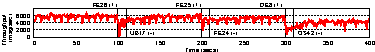
\includegraphics[width=\textwidth]{images/gnuplot/vagrant/reconfiguration/reconfiguration_state10mbs.pdf}\label{fig:s10mbs}}
\subfloat[KVS state size $\approx 60$MBs.]{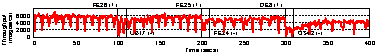
\includegraphics[width=\textwidth]{images/gnuplot/vagrant/reconfiguration/reconfiguration_state50mbs.pdf}\label{fig:s50mbs}}
\caption{KVS performance with \system-triggered reconfigurations on a 50/50 YCSB workload and 1kB-values.}
\label{fig:reconfiguration}
\end{figure}



\textbf{Results:}
Figure~\ref{fig:reconfiguration} shows two types of performance drops.
The first type happens at every 1000 writes and is due to the state checkpoints used to trim the operation logs.
The second type is more severe and less frequent, and happens during reconfigurations, mostly due to the state transfer to the new replica joining the system.
These types of performance perturbations, which become more severe with bigger states, were already identified, and mitigated in previous works~\cite{Bessani:2013}.\footnote{We employ the standard checkpoint and state transfer protocols of BFT-SMaRt and not the one introduced in~\cite{Bessani:2013} as the developers of the system pointed them as more stable.} 

The figure shows that the reconfigurations take around $10$ seconds for these setups, and did not change significantly with states of approx. $30$ and $60$ MBs.
Regarding diversity, the figure shows no noticeable disruption when changing Ubuntu 17 to Fedora 26 and Fedora 25 to Fedora 24, but the replacement of a Debian 8 by an OpenSuse 42 replica significantly decreases the performance, which is consistent with the results from Figure~\ref{fig:bftsmart}.

\subsection{Booting time}

Before triggering a reconfiguration, \system needs to start the new \gls{vm}, boot the \glspl{os}, and launch the BFT-SMaRt replica.
Therefore, the total time to replace a ``risky'' replica roughly comprises the time required to boot the new OS plus the reconfiguration time (discussed in the previous section).
This experiment measures the boot time of the \glspl{os} supported by \system prototype. 

\begin{figure}[h]
\begin{center}
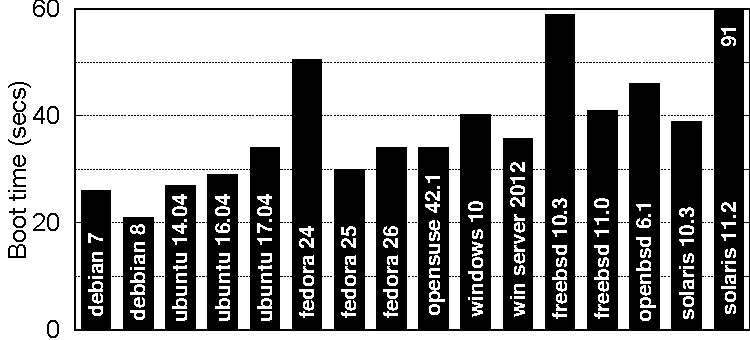
\includegraphics[width=.8\columnwidth]{images/gnuplot/vagrant/updown/boot.pdf}
\vspace{-5mm}
\caption{OSes boot times (seconds).}
\label{fig:boot}
\end{center}
\end{figure}

\textbf{Results:}
Figure~\ref{fig:boot} shows the average boot time of $20$ executions boot for each \gls{os}.
As can be seen, most \glspl{os} take less than 40s to boot, with exceptions of Fedora 24 (50s), FreeBSD 10.3 (59s), and Solaris 11.2 (91s).
In any case, these results together with the reconfiguration times of the previous section show that \system can react to a new threat in less than two minutes (in the worst case).

\subsection{Application Benchmarks}
Our last set of experiments aims to measure the throughput of three existing \gls{bft} services built on top of BFT-SMaRt when running in \system.
The considered applications and workloads are:

\begin{itemize}

\item \emph{KVS} is the same BFT-SMaRt application employed in Section~\ref{sec:reconfiguration}.
It represents a consistent non-relational database that stores data in memory, similarly to a coordination service (an evaluation scenario used in many recent papers on \gls{bft}~\cite{Liu:2016,Behl:2017}).
In this evaluation, we employ the \gls{ycsb} $50\%/50\%$ read/write workload with values of 4k bytes.

\item \sieveq~\cite{Garcia:2016} is a \gls{bft} message queue service that can also be used as an application-level firewall, filtering messages that do not comply with a pre-configured security policy.
Its architecture, based on several filtering layers, reduces the costs of filtering invalid messages in a BFT-replicated state machine.
In our evaluation, we consider all the layers were running on the same four physical machines as the diverse BFT-SMaRt replicas (under different OSes).
The workload imposed to the system is composed of messages of 1k bytes.

\item \emph{BFT ordering for Hyperledger Fabric}~\cite{Sousa:2018} is the first \gls{bft} ordering service for Fabric~\cite{Androulaki:2018}. 
Fabric is an extensible blockchain platform designed for business applications beyond the basic digital coin.
The ordering service is the core of Fabric, being responsible for ordering and grouping issued transactions in signed blocks that form the blockchain.
In our evaluation, we consider transactions of 1k bytes, blocks of $10$ transactions and a single block receiver.

\end{itemize}

As in Section~\ref{sec:performancediversity}, we run the applications on the fastest and slowest diverse replica sets and compare them with the results obtained in bare metal.

\textbf{Results:}
Figure~\ref{fig:apps} shows the peak sustained throughput of the applications. 
The \gls{kvs} results show a throughput of 6.1k and 1.2k ops/sec, for the fastest and slowest configurations, respectively.
This corresponds to $86\%$ and $18\%$ of the 7.1k ops/sec achieved on bare metal.

The \sieveq results show a smaller performance loss when compared with bare metal results.
More specifically, \sieveq in the fastest replica set reaches $94\%$ of the throughput achieved on the bare metal.
Even with the slowest set, the system achieved $53\%$ of the throughput of bare metal.
This smaller loss happens due to the layered architecture of \sieveq, in which most of the message validations happen before the message reaches the \gls{bft} replicated state machine (which is the only layer managed by \system).

The Fabric ordering service results show that running the application on \system virtualization infrastructure lead to $91\%$ (fastest set) to $39\%$ (slowest set) of the throughput achieved on bare metal. 

Nonetheless, even the slowest configurations would not be a significant bottleneck if one takes into consideration the current performance of Fabric~\cite{Sousa:2018}
%Overall, the relatively poor results for the slowest set are due to the single-core and low-memory setups of their replicas (see Table~\ref{tab:oses}).

\begin{figure}[t]
\begin{center}
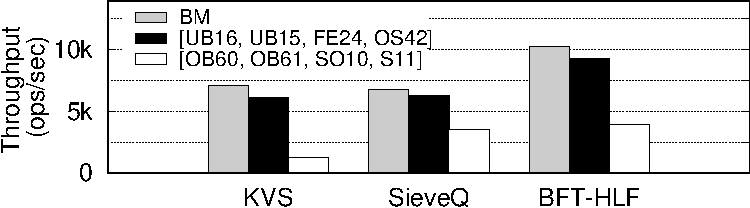
\includegraphics[width=\columnwidth]{images/gnuplot/vagrant/runs_apps/throughput.pdf}
\vspace{-5mm}
\caption{Different BFT applications running in the bare metal, fastest and slowest OS configurations.}
\vspace{-3mm}
\label{fig:apps}
\end{center}
\end{figure}



\section{Final Remarks}
\label{sec:finalremarkslazarus}

\system addresses the long-standing open problem of evaluating, selecting, and managing the diversity of a \gls{bft} system to make it resilient to malicious adversaries.
Our work focuses on two fundamental issues: how to select the best replicas to run together given the current threat landscape, and what is the performance overhead of running a diverse \gls{bft} system in practice.

